\documentclass[a4paper,oneside]{book}

  \usepackage{graphicx}
  \usepackage{xcolor}
  \usepackage{amsmath}
  \usepackage{hyperref}
  
  \usepackage[cm]{fullpage}
  \usepackage{booktabs}
  
  \usepackage{lmodern} 
  \usepackage[T1]{fontenc}
  \usepackage{amsmath}

\begin{document}
  \section*{The hypothetical adaptive value of the generalized growth arrest and the constraints for a successful sex event}
    Molecular, biophysical and chemical data all unequivocally show that the pennate \textit{P. multistriata}, during events of mating and gametogenesis blocks growth and mitosis for a few days, three in the experiment discussed here, xx in the experiment discussed by Scalco et al.

    To analyze the impact of such response on population dynamics, we developed a simple process-based model of the sexual reproduction event (\textbf{Fig.~\ref{fdyn}}), where net growth is the balance between size-dependent cell proliferation and death.
    Within the model, a cell population (P) that reached the carrying capacity enter the sexual reproduction phase, stopping its growth and suffering for extra mortality due to gametogenesis.
    After a certain number of growth arrest days, P reproduces sexually, and an offspring population (F1) appears and start to proliferates.
    When the growth arrest stops, P resumes its growth.
    During the entire course of the simulation (set to ten days) cell growth is modulated by cell size and by competition over Nitrogen.
    Our fundamental assumption, as will be discussed later, is that parents and daughters cells share a common, exclusive microvolume, so that P and F1 compete for N. This is translated in the model as a decrease in growth rate as the total population (F1 + P) converges toward the carrying capacity.

    We chose gametogenesis-induced extra mortality ($d$), growth rates ratio ($g_{0,P}/g_{0,F_{1}}$), day of appearance ($t_{F_{1}I}$), and duration of the growth block (as the block's end day $t_{GE}$) as salient parameters to explore within the simulation to better understand how event timing impact over F1 survival rate (\textbf{Figs.~\ref{gon1},~\ref{gon2},~\ref{gon3}}).
    The range of variations of the different parameters, as well as the value of the other biological parameters, are reported in \textbf{Table~\ref{tbl1}}.
    We deployed an interactive version of the model at the URL \url{https://arfalas.shinyapps.io/pns_toy/}, code and figures are available on \url{https://github.com/bhym/Stec} ({\color{red} currently private})

    \begin{figure}[h]
      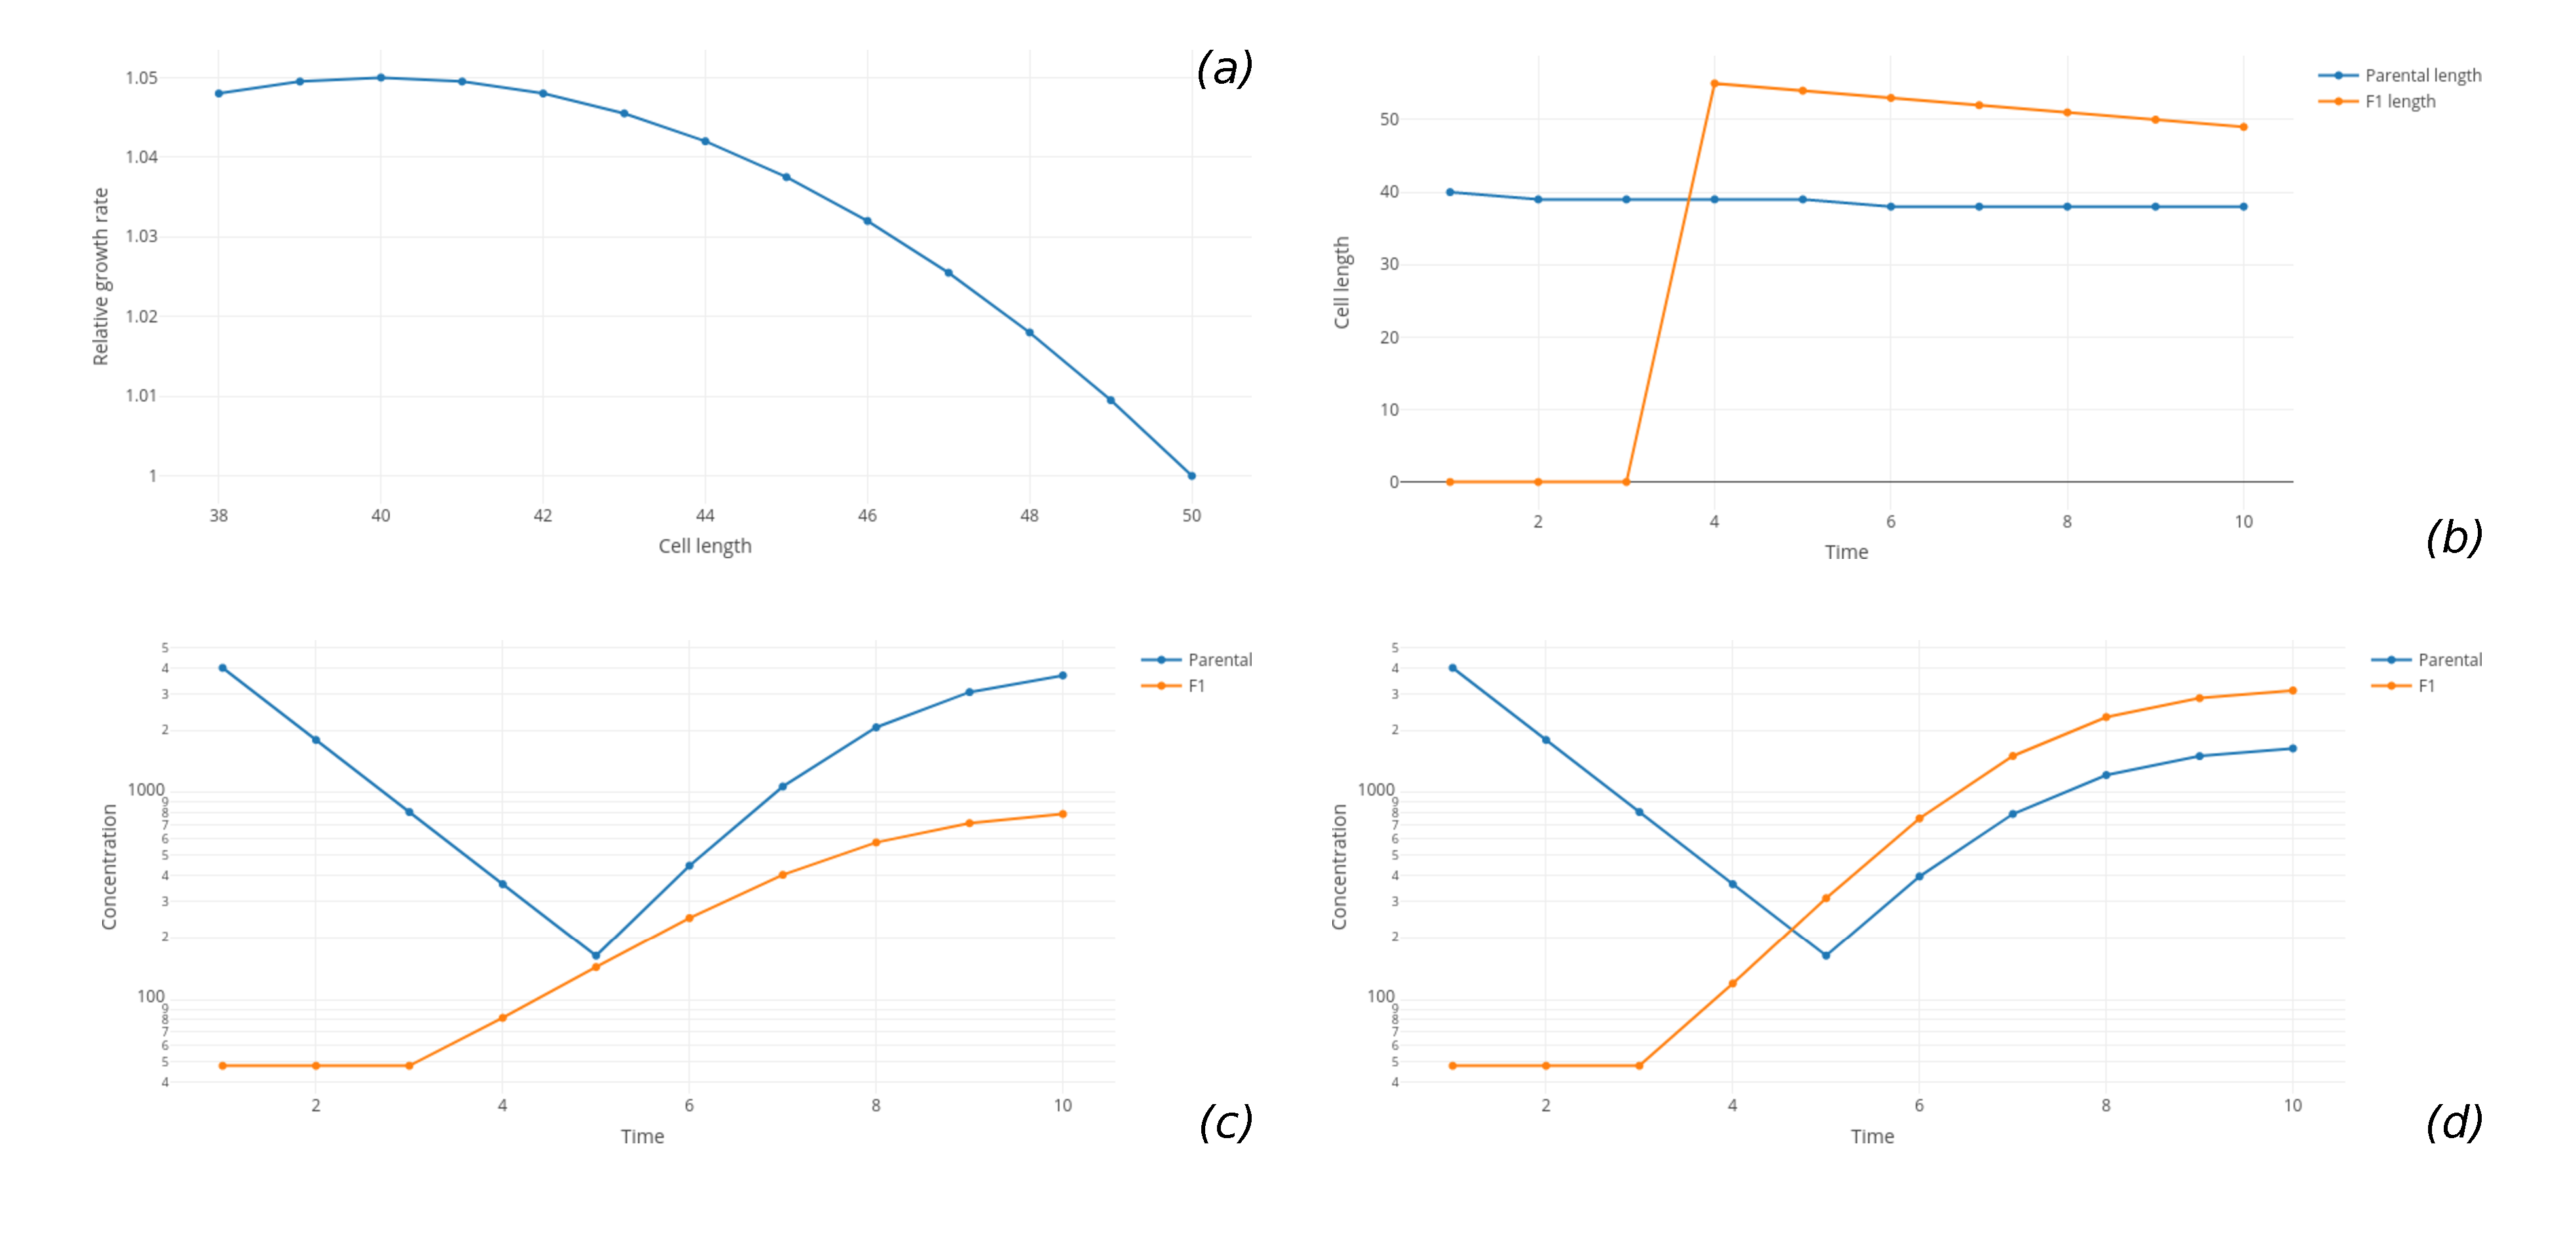
\includegraphics[width=\linewidth]{imgs/Figpan.pdf}
      \caption{\textbf{Time dynamics of the model} --- \textit{(a)} dependence of relative growth rate from length; \textit{(b)} Cell shortening dynamics for the two populations; examples of simulation outputs whith $g_{0,P} >g_{0,F_{1}}$ (1.06 and 0.58, respectively) \textit{(c)} and $g_{0,P} = g_{0,F_{1}}$ \textit{(d)}}\label{fdyn}
    \end{figure}
%
  \section*{Model description}
    Parental ($P$) and offspring ($F1$) dynamics are defined as ODE:\@
    %
    \begin{align}
      \frac{dP}{dt}     &= \kappa \beta_{P}     P - \delta P \\
      \frac{dF_{1}}{dt} &= \kappa \beta_{F_{1}} F_{1}
    \end{align}
    %
    where $\kappa$ is the competition for N, defined as
    \[
      1 - \frac{{[N]}_{t}}{k{[N]}_{t=0}}
    \]
    with 
    \[
      N_{t} = {[P]}_{t} {[N]}_{P} + {[F_{1}]}_{t} {[N]}_{F_{1}}
    \]
    and $k$ as a parameter used to modulate the carrying capacity.

    $\beta_{P}$  and $\beta_{F_{1}}$ are defined as
    \[
      \beta_{P} =
        \begin{cases}
          0               & \mbox{if } t < t_{BE} \\
          \lambda g_{0, P} & \mbox{if } t \geq t_{BE}
        \end{cases}
      \qquad;\qquad
      \beta_{F_{1}} = 
        \begin{cases}
          0                   & \mbox{if } t < t_{F_{1}I} \\
          \lambda g_{0, F_{1}} & \mbox{if } t \geq t_{F_{1}I}
        \end{cases}
    \]
    with $\lambda$ representing allometric scaling on length ($L$), defined as
    \[
      0.25 + 0.04 L_{t} - 0.0005 L_{t}^{2}
    \]
    Length dynamics are based on cell's age ($a$) and are defined by the rule
    \[
      L_{t} = L_{0} - 0.1 a(t)
    \]
    Age is counted from the appearence of the population, and does not increase during GA.\@

    Finally, $\delta$ is an extra mortality term defined as
    \[
      \begin{cases}
        d & \mbox{if } t < t_{BE} \\
        0 & \mbox{if } t > t_{BE}
      \end{cases}
    \]
    
    \subsection*{Parameters}
      \begin{table}
        \caption{Values and ranges for model parameters}\label{tbl1}
         \begin{tabular}{@{}llccr@{}}
          \toprule
            \textbf{Variable}&\textbf{Meaning} & \textbf{Value} & \textbf{Units} & \textbf{Reference}\\
          \midrule
            ${[P]}_{0}$     & initial concentration of P cells           & cells/ml          & 4E3           & The experiment detailed in the paper\\
            $\alpha$        & relative amount of F1 cells                & ---               & 0.012         & The experiment detailed in the paper\\
            $k$             & nitrogen multiplication factor             & ---               & 1.2           & ---\\
            $g_{0, P}$      & basal growth rate for parental generation  & $\text{day}^{-1}$ & {[0.1,5]}     & Explored via simulations\\
            $g_{0, F_{1}}$  & basal growth rate for offspring generation & $\text{day}^{-1}$ & 1             & ---\\
            $t_{BE}$        & end day of the growth arrest               & day               & ${[1,9]}$     & Explored via simulations\\
            $t_{F_{1}I}$    & day of appearence of the offspring         & day               & ${[1,9]}$     & Explored via simulations\\
            $d$             & gametogenesis-induced extra mortality      & day               & ${[0.1,0.9]}$ & Explored via simulations\\
            $L_{0,P}$       & starting length for P cells                &$\mu$m             & 40            & The experiment detailed in the paper\\
            $L_{0,{F_{1}}}$ & starting length for P cells                &$\mu$m             & 55            & The experiment detailed in the paper\\
            $minlen$        & length lower limit for cell division       &$\mu$m             & 38            & D'Alelio et al. (2009)\\
          \bottomrule
        \end{tabular}
      \end{table}
%
  \section*{Results}
    \begin{figure}
      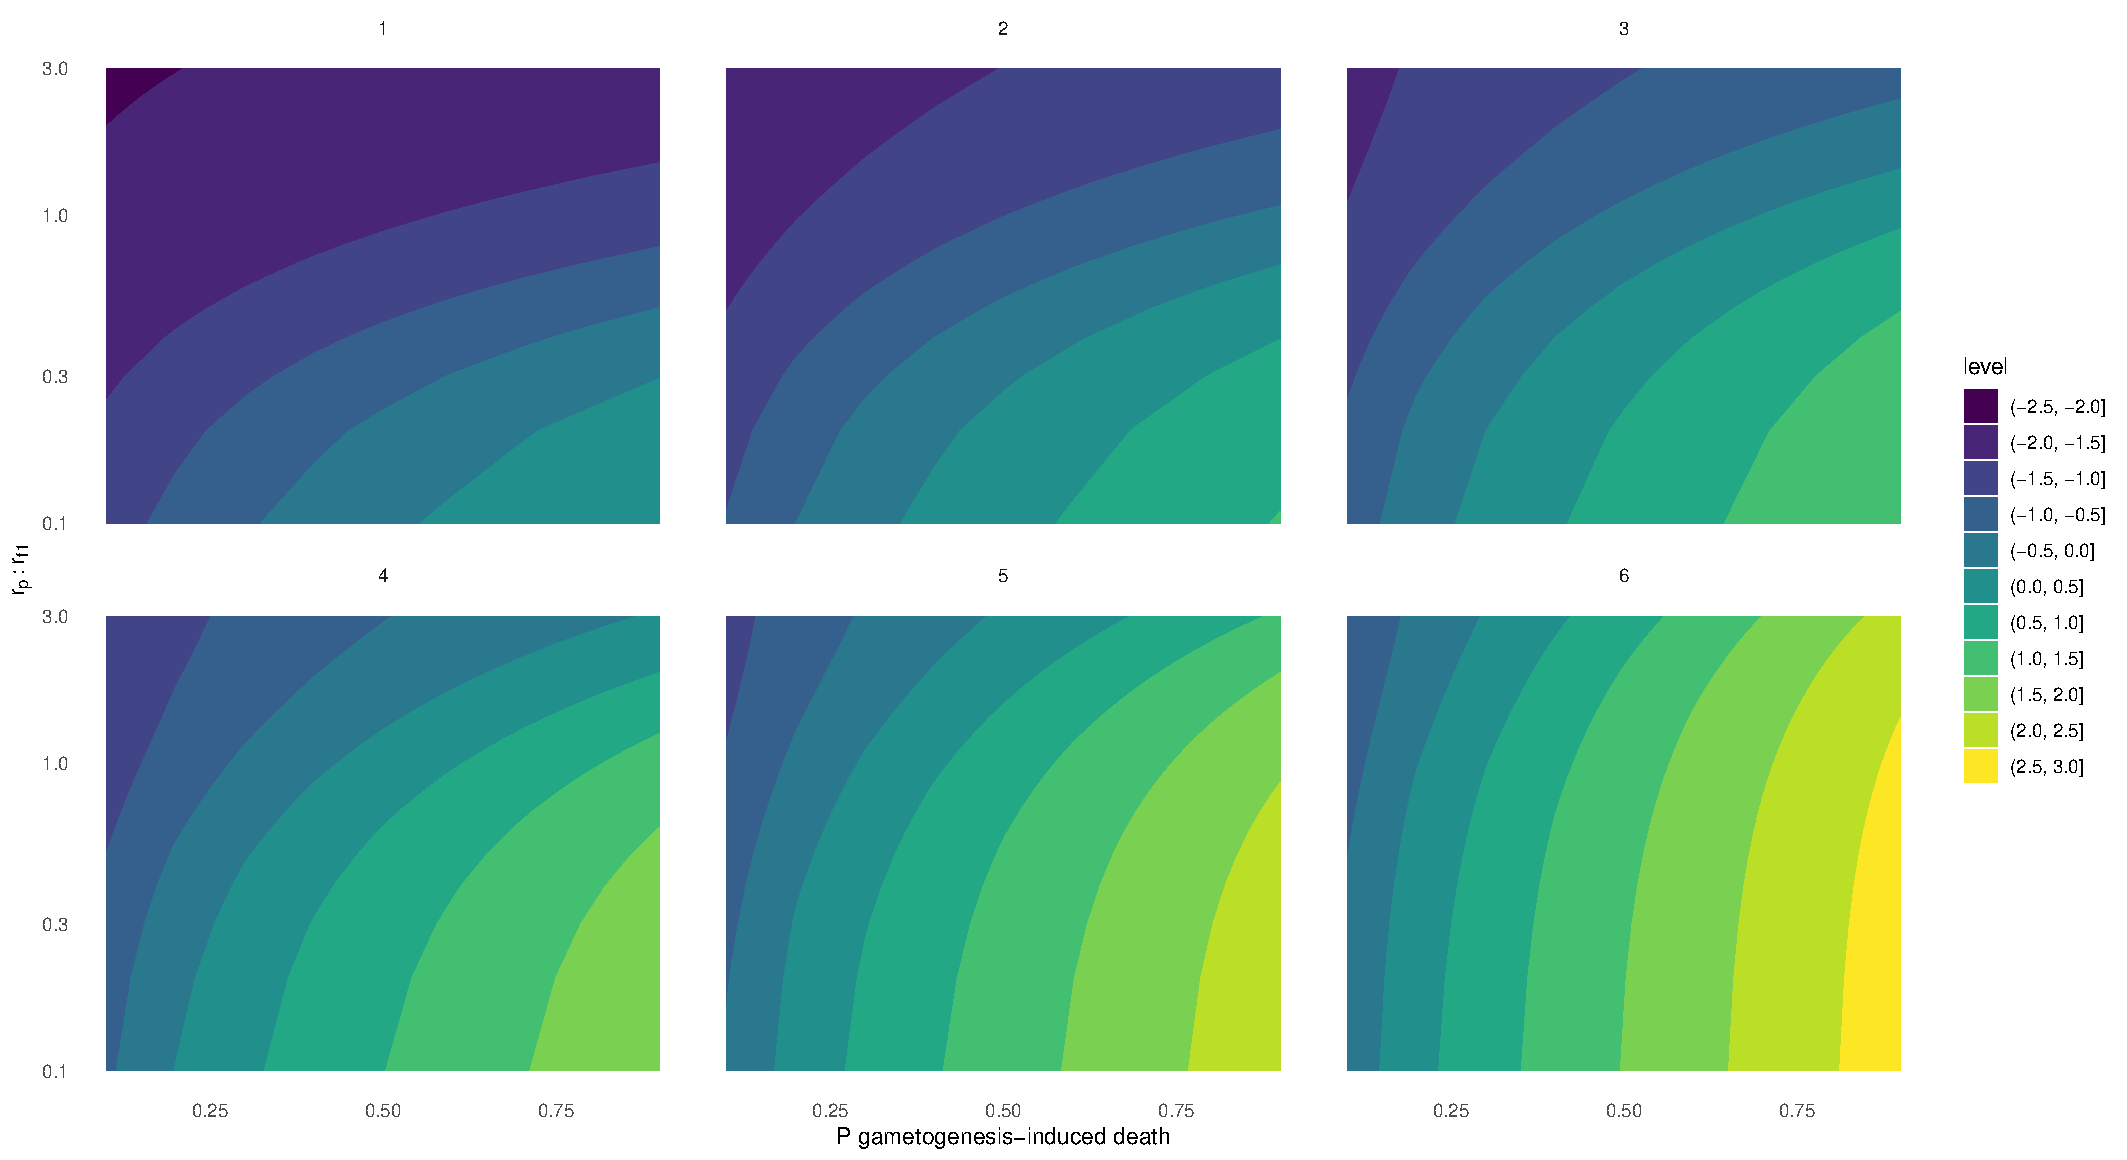
\includegraphics[width=\linewidth]{imgs/a.pdf}
      \caption{\textbf{2D plot of ranges of biomass ratio between P and F1} after 10 days of simulation for paired values of parameters (axes labels). Subplots represent growth arrests of different length.}\label{gon1}
    \end{figure}

    \begin{figure}
      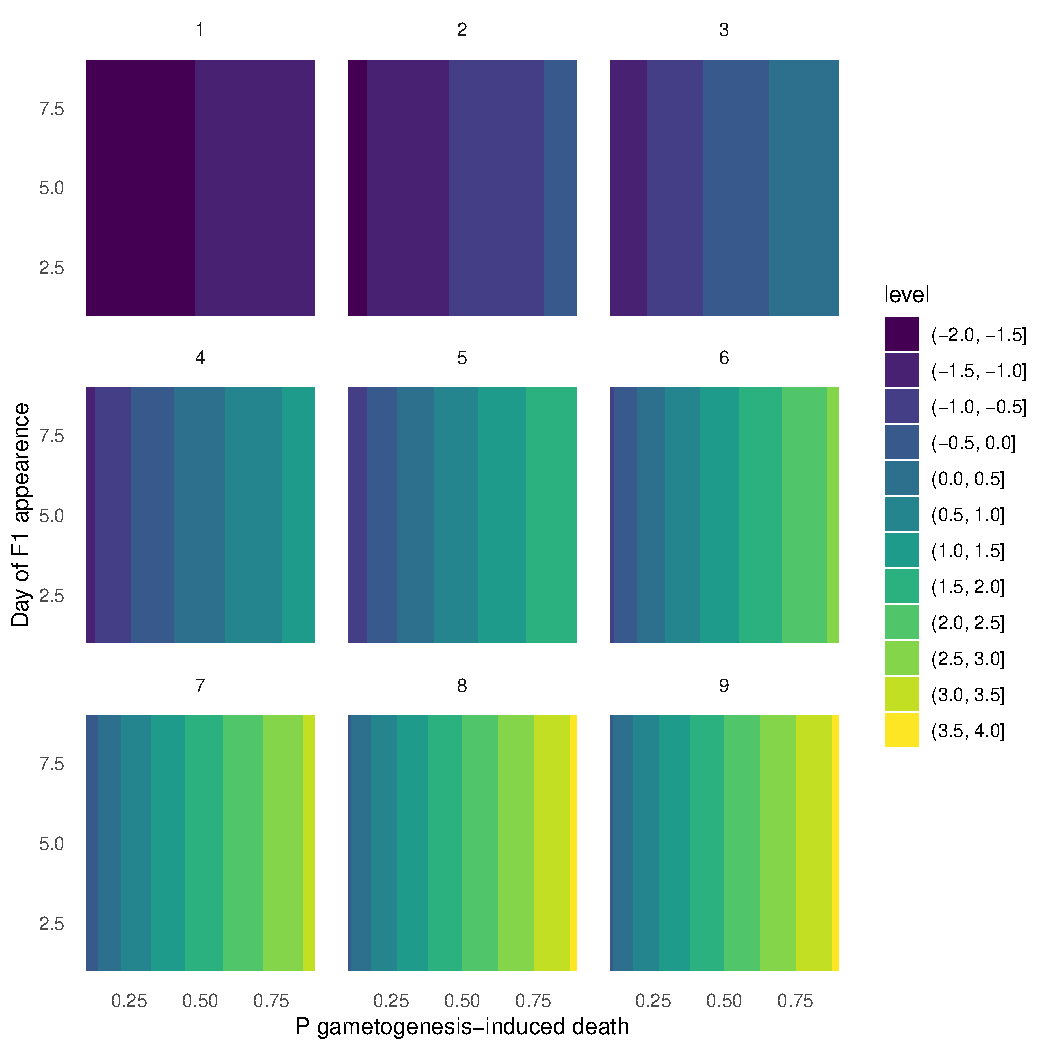
\includegraphics[width=\linewidth]{imgs/b.pdf}
      \caption{\textbf{2D plot of ranges of biomass ratio between P and F1} after 10 days of simulation for paired values of parameters (axes labels). Subplots represent growth arrests of different length.}\label{gon2}
    \end{figure}

    \begin{figure}
      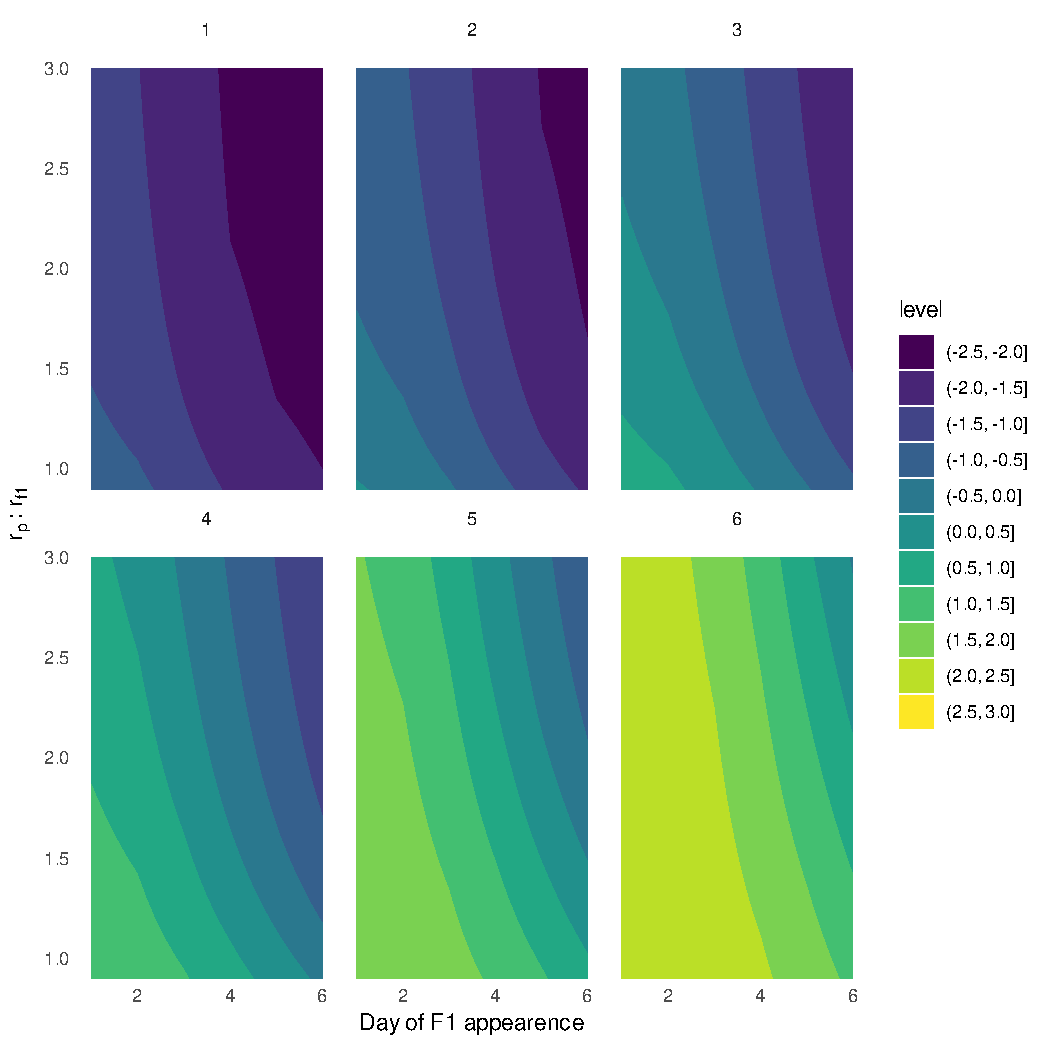
\includegraphics[width=\linewidth]{imgs/c.pdf}
      \caption{\textbf{2D plot of ranges of biomass ratio between P and F1} after 10 days of simulation for paired values of parameters (axes labels). Subplots represent growth arrests of different length.}\label{gon3}
    \end{figure}



Assumptions: 
1. I assume that net growth rate is the balance between size-dependent cell proliferation and death
2. I assume that P suffers extra mortality during growth arrest due to gametogenesis
4. I assume that lenght decreses 1 um after each division
5. I assume that P has reached the environmental carrying capacity before starting the simulation
\end{document}
